\documentclass[tikz,border=0.1cm]{standalone}
\usetikzlibrary{arrows.meta}

\begin{document}
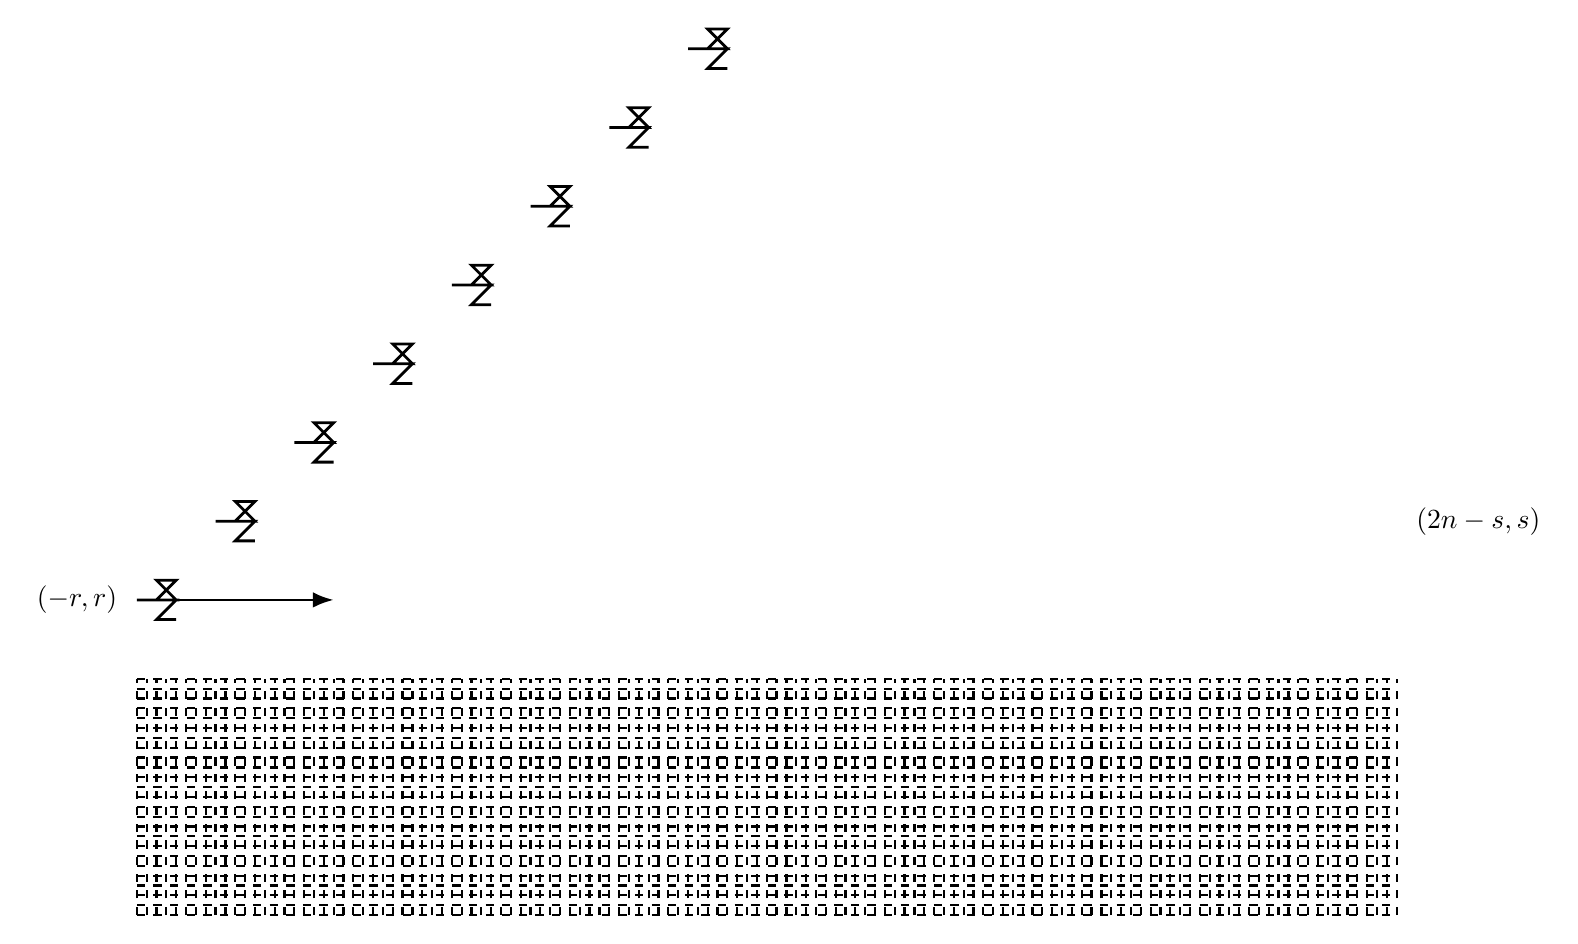
\begin{tikzpicture}[scale=1]
    \draw[thick,xstep=1/8,ystep=1/8,yshift=-1/16,dashed]
        (0,0)
        grid +(16,-3);
    \foreach \i [count=\j] in {0,...,7} {
        \draw[line width=1pt]
            (\i,\j)
            -- ++(0.5,0)
            -- ++(-0.25,0.25)
            -- ++(0.25,0)
            -- ++(-0.25,-0.25)
            -- ++(0.25,0)
            -- ++(-0.25,-0.25)
            -- ++(0.25,0);
        }
    \draw[->,>=Latex,line width=1pt]
        (0.5,1) -- ++(2,0);
    \node[left] at (-1/8,1) {$(-r,r)$};
    \node[right] at (16+1/8,2) {$(2n-s,s)$};
\end{tikzpicture}
\end{document}